\documentclass[11pt]{article}
\usepackage[margin=.9in]{geometry}
\usepackage{lmodern,amsmath,booktabs,graphicx,xcolor}
\usepackage[colorlinks=true,urlcolor=teal,citecolor=teal]{hyperref}
\title{A quiet funding monitor can miss persistent disturbances\\\large Calendar ablation, review burden and a controlled later-period test}
\author{James Jean\\Independent research}
\date{28 October 2026\\GitHub research manuscript; not peer reviewed}
\begin{document}\maketitle
\begin{abstract}
A monitoring queue must distinguish a temporary disturbance from a sustained change without generating too many reviews. Using 2,123 matched SOFR and EFFR effective dates, this study selects among 18 forward-only robust monitoring rules and evaluates a committed choice on 2024--2026 Q3. Thresholds satisfy an alert-burden budget on unmodified validation history; separate synthetic interventions add ten basis points for one or five observations. The selected rule detects 8 of 17 persistent test interventions, versus 3 of 17 for a fixed comparator, with zero new persistence calls in 17 transient interventions. It flags one of 686 unmodified test days but misses nine persistent scenarios. Calendar correction does not win the declared selection rule. The result supports testing review burden and missed disturbances together. It does not establish live-vintage performance, economic false-positive rates or trading value.
\end{abstract}

\section{The review decision}
The number of flags is an incomplete measure of a monitoring system. A rule can keep a queue almost empty by reacting too slowly or setting its cutoff too high. The operational question is whether an alert distinguishes transient variation from a change that persists long enough to justify review.

SOFR and EFFR provide a public setting for investigating that tradeoff. Their administrator describes their construction, publication and revision practices \cite{rates}. This study evaluates a deliberately narrow monitoring design rather than labeling historical dates as financial crises. A controlled intervention makes the target disturbance explicit and repeatable, while measured background history supplies changing conditions. The contribution is an inspectable budget-and-persistence comparison; no new algorithm or exhaustive literature-gap claim is made.

\section{Source, accounting and information boundary}
The original sources are \emph{Secured Overnight Financing Rate} and \emph{Effective Federal Funds Rate}, Federal Reserve Bank of New York. Bounded public API queries retrieve current historical records from 2 April 2018 through 30 September 2026. The responses contain 2,123 SOFR rows and 2,135 EFFR rows, each unique by effective date. SQL retains the 2,123 matching dates and accounts for twelve EFFR-only dates. No missing rate is interpolated.

The analyzed spread is $100(\mathrm{SOFR}-\mathrm{EFFR})$ basis points, where the original rates are percentages. Raw JSON, retrieval timestamps, exact queries and hashes are retained. The source indicators in these responses contain no marked revisions, but that is not evidence that every historical value is unrevised. The API snapshot cannot reconstruct initial intraday publication values. Results therefore concern a retrospective published-history experiment, not demonstrated performance at the first release time.

Original content retains the New York Fed attribution and reuse conditions \cite{terms}. Spreads, adjustments, monitor outputs, figures and interventions are modifications by this project, with no endorsement implied. No private account or participant-level transaction data are used.

\section{Prespecified monitoring and selection}
Initialization uses history through 2021; validation covers 2022--2023. The protected final period is 2024--2026 Q3. Each date's current spread can trigger triage, while all adaptive centers, scales and calendar effects use earlier observations only.

The eighteen candidates cross trailing windows of 30, 60 and 120 observed-rate dates; EWMA weights 0.1, 0.3 and 0.6; and calendar correction off or on. The correction is the historical median difference between month-end-window and ordinary-day spreads, estimated from up to 756 preceding observations with at least ten per group. The calendar window includes a month's last observed rate date and its adjacent observed dates. This uses a retrospective business-day sequence; it is not a claim to anticipate unannounced closures.

For calendar-adjusted spread $x_t$, the standardized deviation and smoothed score are
\[
 z_t=\frac{x_t-\operatorname{median}(x_{t-w:t-1})}
 {\max\{1,1.4826\operatorname{median}|x_{t-w:t-1}-\operatorname{median}(x_{t-w:t-1})|\}},
 \qquad e_t=\alpha z_t+(1-\alpha)e_{t-1}.
\]
The scale floor is one basis point, a declared engineering choice preventing division by nearly constant history. A persistent flag requires $|e_t|$ and $|e_{t-1}|$ both to exceed a cutoff. The initial score is zero.

Each candidate tests cutoffs 0.5, 1, 1.5, 2, 3, 4, 6 and 8 on unmodified validation days. It selects the smallest meeting an at-most-1\% flag budget; candidates with no qualifying cutoff explicitly issue no flags. This is a review-burden constraint on unlabeled data, not a measured economic false-positive rate.

Separate validation interventions start every forty observations after a twenty-observation offset, leaving seven observations for scoring. Each adds ten basis points to SOFR alone for one observation or five observations. The monitor adapts to earlier injected observations. A detection requires a new persistent flag beyond the unmodified monitor during the seven-observation window. This prevents an existing background flag from silently counting as an intervention hit.

Selection maximizes persistent detection fraction minus transient persistent-call fraction, then lower background burden and candidate name. The winner is window 30, alpha 0.6, no calendar correction and cutoff 6. The fixed comparator is window 60, alpha 0.3, no correction and its own validation-calibrated cutoff 6. All trials, cutoffs, outcomes and runtimes are retained. The winner uses the smallest tested window and largest smoothing weight; the finite grid establishes no global optimum. Selection was committed before the test command.

\section{Later-period results}
\begin{table}[ht]\centering
\caption{Frozen rules on 686 unmodified test observations and separate synthetic interventions.}
\begin{tabular}{lrr}\toprule
Measure & Selected & Comparator\\\midrule
Unmodified days flagged & 1 & 0\\
Five-observation interventions detected & 8/17 & 3/17\\
One-observation interventions producing new persistence & 0/17 & 0/17\\
Median delay among detected persistent cases & 1.5 & 3.0\\\bottomrule
\end{tabular}\end{table}

The selected rule detects six persistent cases that the comparator misses; the comparator detects one that the selected rule misses. Its net improvement is five of the seventeen declared cases. It still misses nine, and both rules make no new persistent calls in the seventeen transient cases. Zero observed transient calls is not proof of a zero error probability.

The selected rule's one background flag corresponds to 0.15\% of the unmodified test observations. Such a low queue burden can coexist with incomplete detection. Conditional delay medians concern different successful-case subsets and should not be presented as a paired speed advantage. Case dates, individual successes, misses, delays and background indicators remain available for inspection.

\begin{figure}[ht]\centering
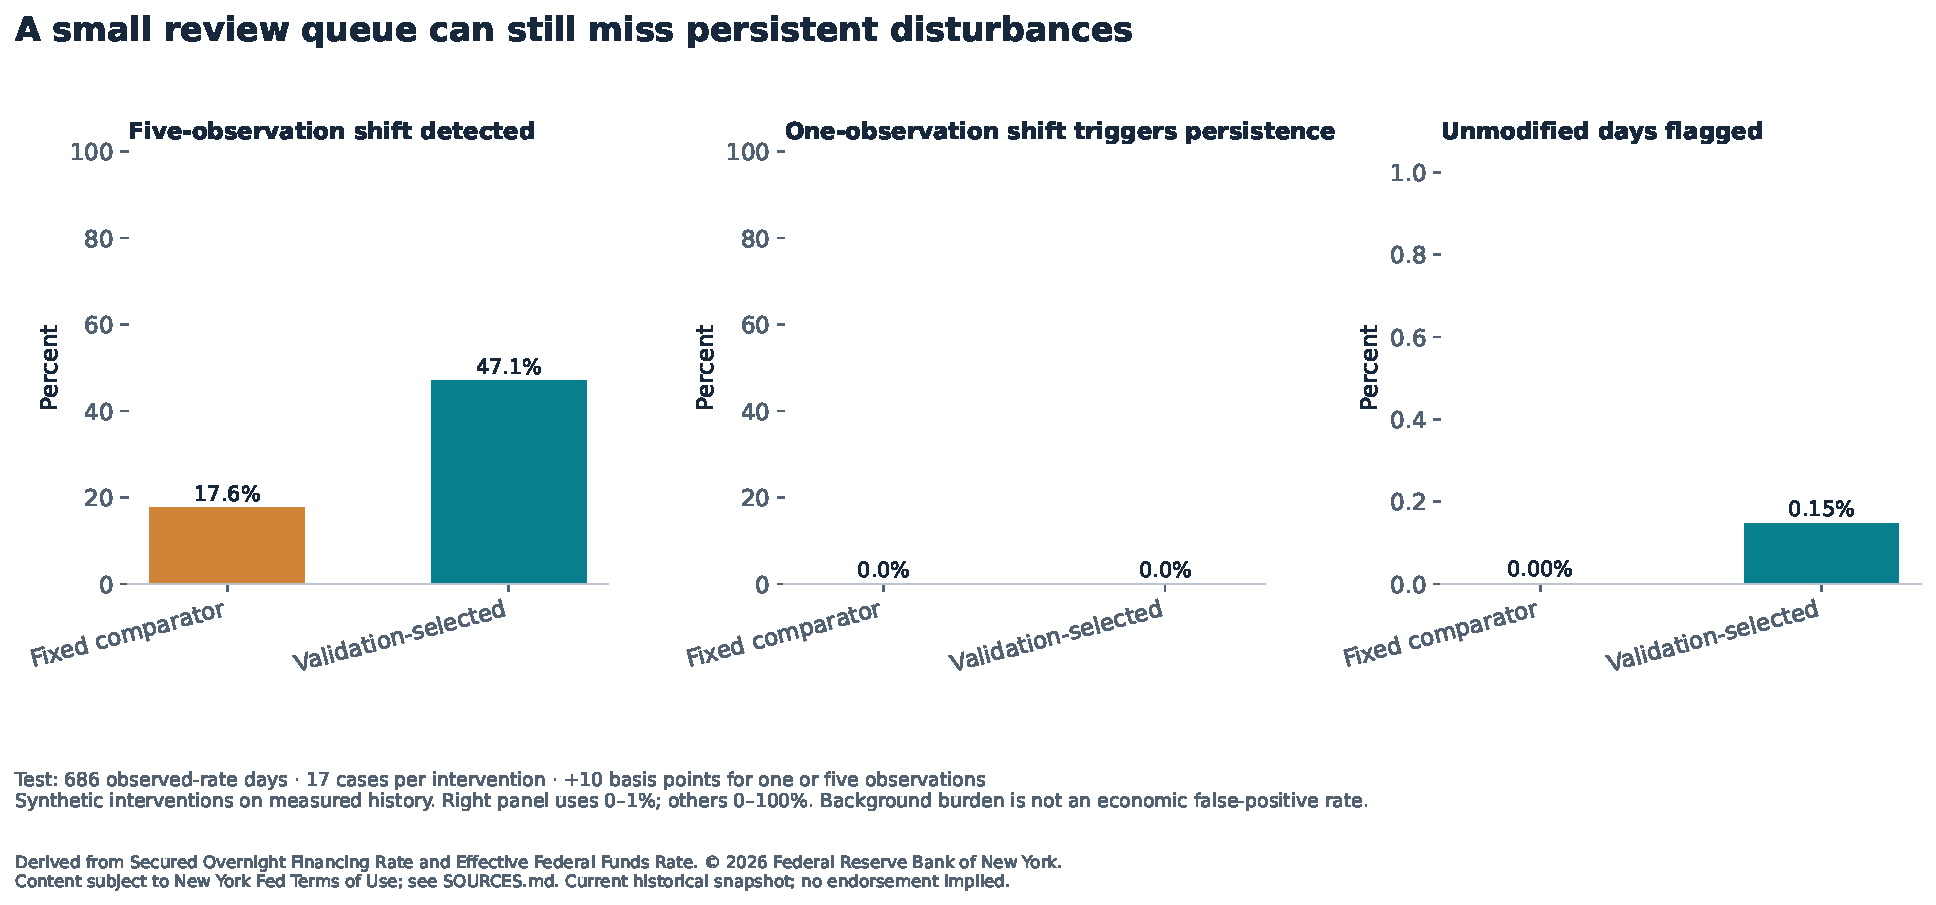
\includegraphics[width=\linewidth]{images/decision-summary.pdf}
\caption{Detection and review burden answer different questions. Interventions are synthetic scenarios imposed separately on measured history; the right panel uses a different percentage scale.}
\end{figure}

The interventions reuse historical monitoring state and are not independent economic episodes. Accordingly, this study reports finite-case counts rather than a confidence interval that treats the scenarios as independent trials. The outcome is conditional on the chosen disturbance size, duration, start schedule and historical snapshot. It cannot establish a production detector's crisis sensitivity or false-positive rate.

\section{Checks and next experiment}
A separate verifier imports no monitoring helpers. Standard-library median arithmetic recomputes every exported center, scale, calendar correction, EWMA, flag, intervention outcome and delay. Original hashes, exact joins, basis-point conversions, calendar flags, cutoff choices and model selection reconcile. Five contract tests cover future-input independence, two-observation persistence, the scale floor, cached-state equivalence to full recalculation and the explicit no-alert policy. A full offline replay regenerates all eighteen trials and protected test outcomes.

Two implementation details were corrected transparently: the terminal calendar-date flag was repaired before test evaluation, and the independent verifier learned to parse nullable CSV delays represented as decimal strings. Neither correction changes a search objective or chooses a policy using test outcomes.

The next experiment should retain publication vintages and independent episode annotations, then compare review burden, missed episodes and delay under agreed operating costs. Alternative disturbance sizes and directions require a fresh declared evaluation rather than retrospective threshold selection. This study supports that experimental design; it makes no trading, profitability or economic causal claim.

\section*{Reproducibility and attribution}
Public source snapshots, SQL, code, complete trials, outcomes, figures and independent checks are at \href{https://github.com/S3R3Bii/funding-alert-burden}{the study repository}. This research manuscript is shared on GitHub and has not been peer reviewed. AI assisted coding and drafting. Measured history, synthetic scenarios and proposed next experiments are identified separately.

\noindent\small\copyright\ 2026 Federal Reserve Bank of New York. Content from the New York Fed subject to the Terms of Use at newyorkfed.org. Derived analyses are this project's work; no endorsement is implied.\normalsize
\begingroup\small\begin{thebibliography}{9}\setlength{\itemsep}{2pt}
\bibitem{rates} Federal Reserve Bank of New York. Additional Information about Reference Rates Administered by the New York Fed. Accessed 28 October 2026. \href{https://www.newyorkfed.org/markets/reference-rates/additional-information-about-reference-rates}{Source methodology and revision practices}.
\bibitem{terms} Federal Reserve Bank of New York. Terms of Use. \url{https://www.newyorkfed.org/privacy/termsofuse}.
\end{thebibliography}\endgroup\end{document}
